\chapter{Smitc solver -- 2D -- Deflection of a linear elastic plate}

\modinfo{Directory}{ElasticPlateLinear}
\modinfo{Solvers}{\Idx{SmitcSolver}} 
\modinfo{Tools}{\Idx{ElmerGUI}} 
\modinfo{Dimensions}{2D, Eigenmode}
\modinfo{Author}{Peter R{\aa}back}


\subsection*{Problem description}

This tutorial demonstrates how to use the Smitc solver to solve small deflections of plates.
The Smitc solver is for elastic linear plates and uses the theory of Reissner and Mindlin.

The case under investigation is a L-shaped steel plate under pressure.
The plate is shown in figure~\ref{fig:simplePlate}
The longer sides have the length of $2\,m$ and the shorter $1\,m$. 
So the area of the plate is $3\,m^2$. The plate has a thickness of
$1\,cm$. We assume that on the plate
there is about $15300\,kg$ of sand. The sand is uniformly distributed
on the plate and the sand stays uniformly distributed even if the 
plate undergoes small deflection. The sand exerts to the plate
a pressure of $50000\,Pa$. The plate is clamped from all sides
meaning that both deflection and rotation are zero on all edges.
%
\begin{figure}[tbhp]
\begin{center}
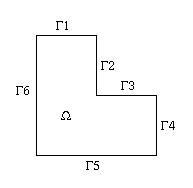
\includegraphics[width=0.4\textwidth]{simplePlate}
\end{center}
\caption{The geometry of plate and the numbering of edges.}
\label{fig:simplePlate}
\end{figure}


For more details on the solver we refer to the documentation of Smitc solver in the 
Elmer Models Manual.

\subsection*{Solution procedure}

Start \texttt{ElmerGUI} from command line or by clicking the icon in your desktop. Here we describe 
the essential steps in the ElmerGUI by writing out the clicking procedure. Indentation generally means that the 
selections are done within the window chosen at the higher level. 

Before we can start the set-up we should make sure that the menus for Smitc solver are present.
If not, they may be found in file
\ttbegin
$ELMERHOME/bin/edf-extra/elasticplate.xml
\ttend
To load these definitions do the following
\ttbegin
File
  Definitions
    Append -> choose the file
\ttend
To see what kind of new menu structures were loaded you may play around with viewer collapsing and opening. 
Note that if you want to load an existing project you should load the xml-definitions that were used 
in creating the project. Therefore it may be best to place all actively used menu definitions in directory
\ttbegin
$ELMERHOME/bin/edf
\ttend

When the menu structures for plate solver are there then we are ready to continue.
The first thing to do is create a mesh with ElmerGrid.
The definition of mesh is in the file \texttt{simple\_plate.grd}.
The mesh is about uniform and consist of 1000 linear square elements.
\ttbegin
File 
  Open -> simple\_plate.grd
\ttend

You should obtain a L shaped figure with 6 sides.  You may check in the \texttt{Model summary...} 
window that it consists of 1082 nodes and 1008 surface elements.
If the mesh was successfully imported your window should look 
something like figure~\ref{fig:simplePlateMesh}.
%
\begin{figure}[tbhp]
\begin{center}
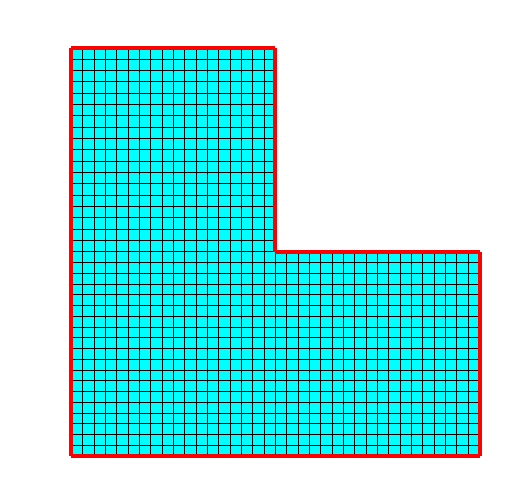
\includegraphics[width=0.48\textwidth]{simplePlateMesh}
\end{center}
\caption{The plate mesh}
\label{fig:simplePlateMesh}
\end{figure}




After we have the mesh we start to go through the Model menu from the top to bottom. 
In the \texttt{Setup} we choose things related to the whole simulation such as file names, 
time stepping, constants etc.

The simulation uses 2D Cartesian geometry. The simulation is not time dependent
i.e. Steady State.  There are no coupled solvers so only one iteration is needed.  
\ttbegin
Model
  Setup 
    Simulation Type = Steady state
    Steady state max. iter = 1
    Apply
\ttend

In the equation section we choose the relevant equations and parameters related to their solution. 
When defining Equations and Materials it is possible to assign to the bodies immediately, or to use mouse
selection to assign them later. In this case we have just one body and therefore its easier to assign 
the Equation and Material to it directly.


\ttbegin
Model
  Equation
    Add 
      Name = Elastic Plate
      Apply to bodies = 1
      Elastic Plates
        Active = on           
    Add  
    OK
\ttend        

The Material section includes all the material parameters.
They are divided into generic parameters which are direct properties of the material
without making any assumptions on the physical model, such as the mass. Other properties assume
a physical law, such heat Young's modulus. As our problem is academic in nature we choose some 
simple ideal parameters, similar to steel, but data from material database could also be used instead.
\ttbegin
Model
  Material
    Add 
      Name = Ideal
      Apply to bodies = 1 
      General    
        Density = 7800.0
      Elastic Plates
        Youngs Modulus = 209.0e9
        Poisson ratio = 0.3
        Thickness = 1.0e-2
        Tension = 0.0	
      Add
      OK
\ttend

A Body Force represents the right-hand-side of a equation i.e. 
external forces. In Body Force block we give the equations right hand side. 
It is the uniform pressure from the weight of the sand and it is 
the same constant in every point.
\ttbegin
Model
  BodyForce
    Name = Pressure
    Apply to Bodies = Body 1 
    Elastic Plates 
      Pressure = 5.0e4
    Add
    OK
\ttend


In this case all the boundaries are rigidly fixed we set all the components of the 
solution field to be zero. The 1st component is the displacement in the normal direction
while the 2nd and 3rd components  are actually the components of rotation vector
\ttbegin
Model
  BoundaryCondition
    Add 
      Elastic Plates
        Deflection 1 = 0.0
        Deflection 2 = 0.0
        Deflection 3 = 0.0
      Name = Fixed
      Apply to boundaries = 1 2 3 4 5 6
      Add
      OK
\ttend   

For the execution ElmerSolver needs the mesh files and the command file. 
We have now basically defined all the information for ElmerGUI to write 
the command file. After writing it we may also visually inspect the command file.
\ttbegin
Sif 
  Generate
  Edit -> look how your command file came out  
\ttend

Before we can execute the solver we should save the files in a directory. In saving the project all the
necessary files for restarting the case will be saved to the destination directory.
\ttbegin
File 
  Save Project
\ttend

After we have successfully saved the files we may start the solver
\ttbegin
Run
  Start solver
\ttend
A convergence view automatically pops up showing relative changes 
of each iteration.  In this case there is just one iteration and thus 
no curve appears.  The problem is solved in few seconds.

\subsection*{Results}
To view the results start Paraview
\ttbegin
Run
  Paraview
\ttend
and select the 1st component of the \texttt{deflection} field (confusingly 
named the x-component). 

 Currently you would use Paraview, ElmerVTK, or something that can read the
VTU files. Here the results are shown from Paraview.

Result for displacement (deflection x) is shown in figure~\ref{fig:simplePlateDeflection}.
%
\begin{figure}[tbhp]
\begin{center}
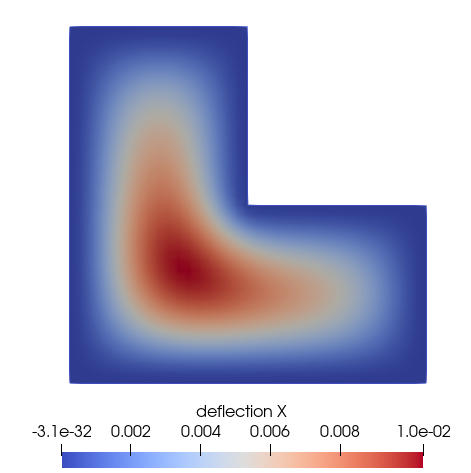
\includegraphics[width=0.48\textwidth]{simplePlateDeflection}
%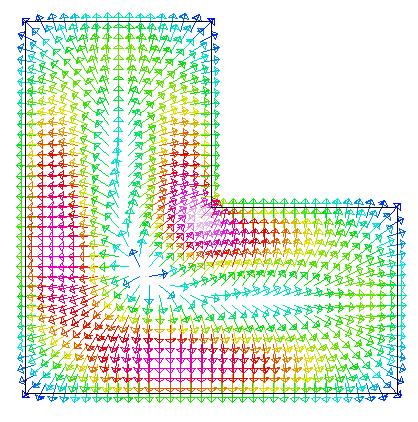
\includegraphics[width=0.48\textwidth]{simplePlateRotation}
\end{center}
\caption{The deflection of the plate.}
\label{fig:simplePlateDeflection}
\end{figure}

Note that the 1st component of Deflection is the displacement to normal
direction whereas the 2nd and 3rd components are the x- and y-components of
rotation vector, and are shown in figure~\ref{fig:simplePlateRotation}.


\begin{figure}[tbhp]
\begin{center}
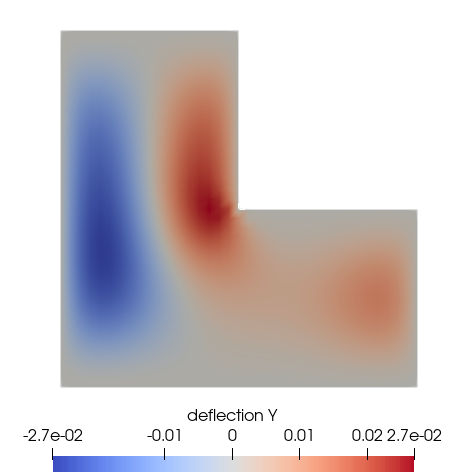
\includegraphics[width=0.48\textwidth]{simplePlateRotationY}
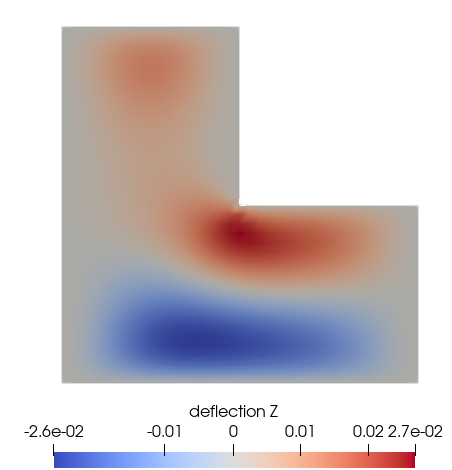
\includegraphics[width=0.48\textwidth]{simplePlateRotationZ}
\end{center}
\caption{The rotation of the plate in x and y components.}
\label{fig:simplePlateRotation}
\end{figure}



\subsection*{Extra task}
You may test the effect of pre-stressing by altering the Tension material parameter.  




\hfill
\mbox{}






